\item Prism 1 with bar 2 of mass \( m \) placed on it gets a horizontal acceleration \( w \) directed to the left (Fig. 1.23). At what maximum value of this acceleration will the bar be still stationary relative to the prism, if the coefficient of friction between them \( k < \cot \alpha \)?
    \begin{center}
        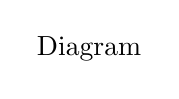
\begin{tikzpicture}
            \node at (0, 0) {Diagram};
        \end{tikzpicture}
    \end{center}